\noindent
% \begin{figure*}[!ht]
%   \begin{center}
%   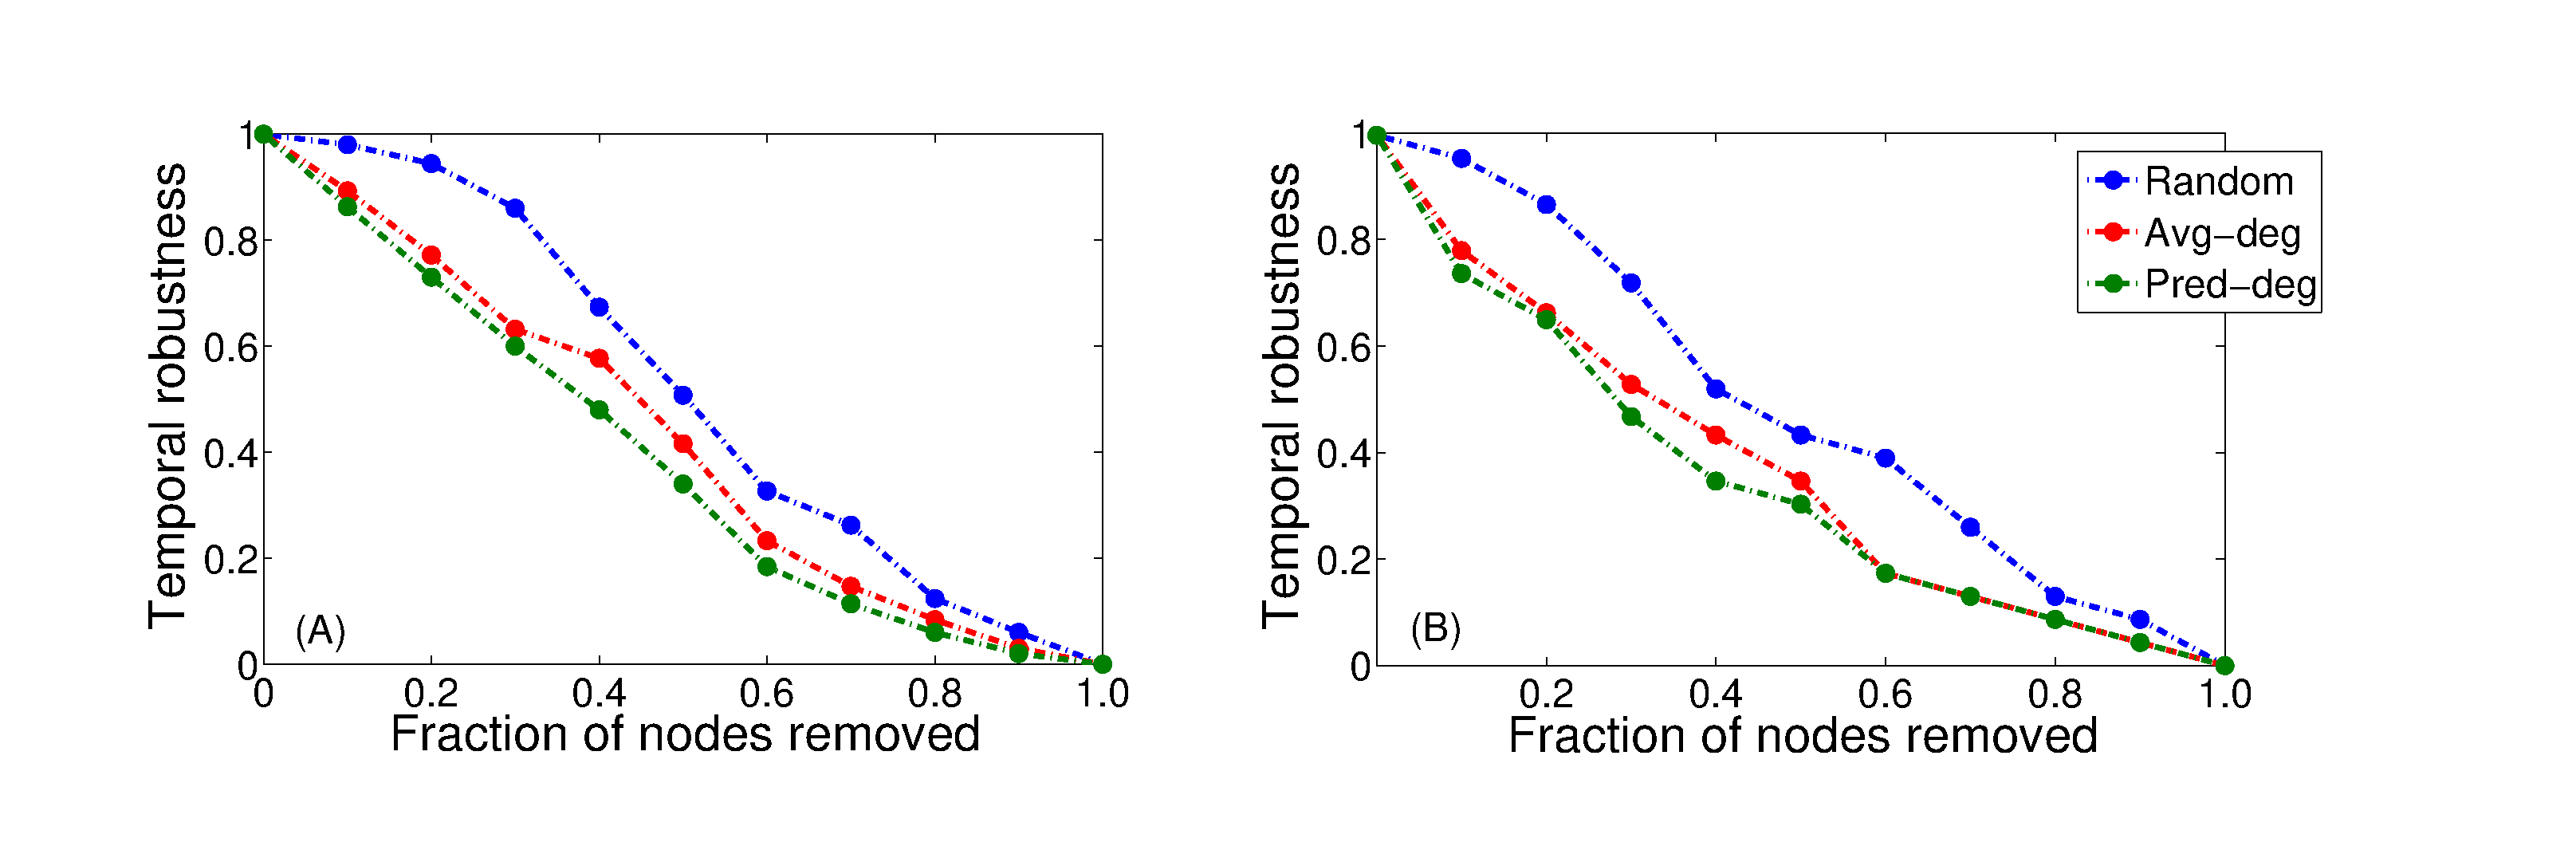
\includegraphics[width=0.9\linewidth, angle=0]{fig/attack_all.eps}
%   \caption{\label{fig_attack}Temporal robustness as a function of the fraction of removed nodes for (a) INFOCOM 2006 and (b) SIGCOMM 2009 datasets.}
%   \end{center}
%  \end{figure*}

\section{An attack strategy using prediction framework}
\label{attack}
%\todo{Be careful to have the window size `w' to be same for all the techniques -- I think thisis not there}
In this section we show how our prediction can be used in order to launch targeted attack on temporal networks. The strategy proposed is a modification over the average node degree attack presented in ~\cite{trajanovski2012error}. 
In case of average node degree attack the temporal degree\footnote{Given a time interval [$t_1, t_n$] temporal degree of node $i$ is the average degree of $i$ over the time interval}  
~\cite{trajanovski2012error} of the nodes are calculated and the node with highest temporal degree is removed in the 
subsequent steps (i.e., ``the node is attacked''). 
We observe that for every 
node its degree over a given time interval forms a time series. Using our prediction framework we calculate the degree of the node at a future time step based on the previous 
$w$ time steps (window size for the corresponding dataset, refer to section \ref{prediction_1})
and remove a node with the 
highest degree as predicted by our proposed framework. We compare our strategy (Pred-deg) with average node degree based attack (Avg-deg) and the random case (nodes are selected at random 
and removed). 
We measure the effectiveness of an attack strategy by using temporal robustness~\cite{trajanovski2012error} which we estimate by the relative change in efficiency~\cite{trajanovski2012error} 
after a structural damage $D$. 
Temporal efficiency of a network $G$ in a given time interval [$t_1,t_n$], $E_G(t_1,t_2)$ is defined as the averaged sum of the inverse temporal distances over all pairs of 
nodes in that time interval. 
\begin{center}
 $E_G(t_1,t_2)=\frac{1}{N(N-1)}\Sigma_{i,j:i\neq j}\frac{1}{d_{ij}(t_1,t_2)}$
\end{center}
Here $N$ is the number of nodes in the network and $d_{ij}(t_1,t_2)$ is the temporal distance which is the smallest temporal length paths among all the temporal
paths between $i$ and $j$ in the time interval [$t_1,t_2$]. Hence, temporal robustness is defined  as $R_G(D)=\frac{E_{GD}}{E_G}$. 
In figure~\ref{fig_attack} we plot temporal robustness 
as a function of the fraction of nodes ($P$) removed 
for (a) INFOCOM 2006 and (b) SIGCOMM 2009 datasets. 
We observe that our strategy 
does better than both the random and average node degree based strategy. 

\if{0}
The reason for this result is straightforward. In the original average node degree based attack one averages 
the degree of a node for $n$ previous time steps and uses the value to rank the nodes of the $(n+1)^{st}$ time step (test data) and removes the top $P$ fraction of nodes. 
In our method, we use the actual degree values of the previous $n$ steps (training data), visualize them as a time series and predict the degree values of the $(n+1)^{st}$ step. The scheme based on 
the predicted degree values (which are pretty accurate estimates of the actual degree values of the $(n+1)^{st}$) is expected to produce a better ranking than the state-of-the-art 
scheme. As an additional advantage spectrogram analysis can also separate out the cases where our strategy would not work. 
Note that similar attack strategies could be developed based on other network properties as well.
We believe that our framework can be used as a better ranking scheme for nodes in a temporal network at a future time instant even if the network structure itself at that time point 
is unknown.
% \begin{figure*}[!ht]
%   \begin{center}
%   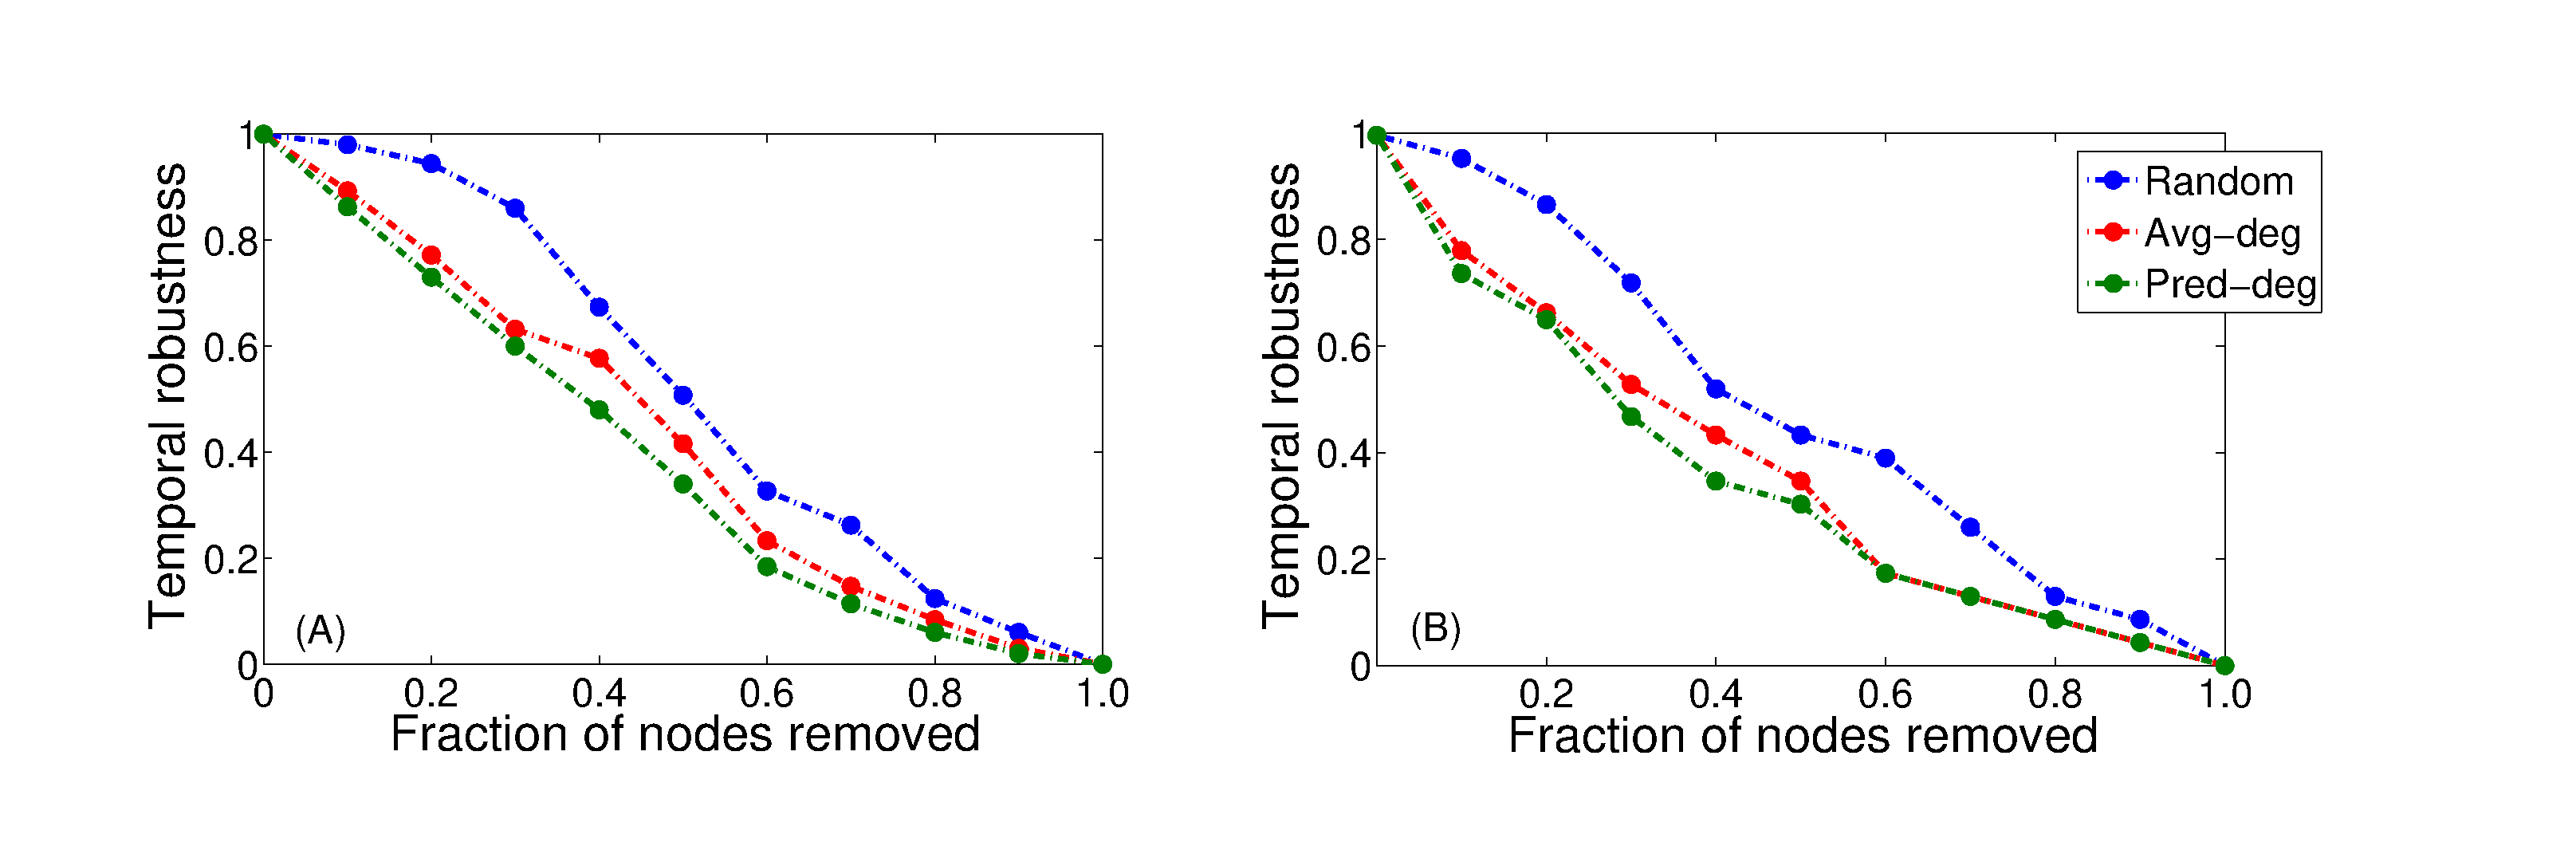
\includegraphics[width=0.9\columnwidth, angle=0]{fig/attack_all.eps}
%   \caption{\label{fig_attack}Temporal robustness as a function of the fraction of removed nodes for (a) INFOCOM 2006 and (b) SIGCOMM 2009 datasets.}
%   \end{center}
%  \end{figure*}
\fi


% \todo{This section is not needed -- remove}
% \subsection{Insights}  
% \label{insights}
% %\textcolor{blue}{
% \begin{itemize}
% %  \item Based on our analysis we can conclude that temporals networks representing human interactions can be sub divided into a two different classes. The datasets INFOCOM 2006 and 
% %  SIGCOMM 2009 which represent human face-to-face interaction differ significantly from the Twitter hashtag co-occurrence and the Facebook posts dataset 
% %  which represent human communication through social media. 
% %  Unlike the previous cases the 
% %  Twitter hashtag co-occurrence network is memory-less and almost no structural correlation exists. 
% %  For Facebook posts network also we find the network to be memory-less with only few of the properties showing presence of auto-correlation.
%  %From our analysis we are able to identify more than one class of temporal networks (we identify at least two here) and also conclude that not all temporal networks show structural 
%  %correlation.
%  \item 
% \todo{ Something like this may come just after prediction - I have diccussed with SS}
% We observe that the structural properties of a temporal network can be classified based on how well they can be predicted. We further observe that for 
%  both the datasets edge-emergence and number of active nodes give the best prediction result while betweenness centrality offers the worst prediction result.
%   This can be attributed to the fact that 
%  a person (node) who is a part of a conversation (network) at a time instant will remain a part of it in the next few time instances with high probability.
%  However, the node being a part of many shortest paths is a far rare event. 
% \todo{If you want you can mention it passingly in the conclusion}
%  \item In its current state our framework can predict the values of the network properties at a future time step but is unable to offer the exact network 
%  structure at that time step. But our framework can have genuine contributions toward link prediction in temporal networks. Since we show that structural 
%  correlation exists in these networks and we can also predict the network properties at these time steps as well, we can re-frame the link prediction problem 
%  as a network at a time step which is obtained from the network at a previous time step with minimal changes made depending on the values of the properties. 
%  We plan to deeply investigate this problem in subsequent works.
% \end{itemize}
% %}

% \subsection{An attack strategy using prediction framework}
% In this section we propose an attack strategy using based on our prediction framework. The strategy proposed is a modification over the average node degree attack. In case 
% of average node degree attack the temporal degree ~\cite{trajanovski2012error} of the nodes are calculated and node with highest temporal degree is attacked. We observe that given a 
% node its degree over a given time interval forms a time series. Using our prediction frame work we calculate the degree of the node at a future time step and remove a node with the 
% highest degree as obtained from the frame work. We compare out strategy (Pred-deg) with average node degree based attack (Avg-deg) and the random case (nodes are selected at random 
% and removed). In figure ~\ref{fig_attack} we plot temporal robustness ~\cite{trajanovski2012error} as a function of the fraction of nodes removed for Infocom 2006 dataset. We observe that our strategy 
% does better than both the random and average node degree based strategy. Note that similar attack strategies could be developed based on other network properties as well.
% 
% \begin{figure}[!ht]
%   \begin{center}
%   \includegraphics[width=0.7\columnwidth, angle=0]{fig/attack.eps}
%   \caption{\label{fig_attack}Temporal robustness as a function of the fraction of removed nodes for Infocom 2006 dataset.}
%   \end{center}
%  \end{figure}


\medskip
